\section{Исследование аттракторов внутренних волн на базе квазигидродинамического подхода}

Предлагается эффективный подход к моделированию аттракторов внутренних волн, который совмещает в себе точность метода спектральных элементов и гибкость реализации метода конечных объемов. Данный подход основан на моделях, которые обобщают уравнения для описания движения течения жидкости и газа. Расширенная, квазигидродинамическая система Навье-Стокса отличается от классической диссипативными слагаемыми. Преимущество состоит в простоте и удобстве численной реализации.

 Разработка квазигидродинамических и квазигазодинамических подходов ведется с восьмидесятых годов сотрудниками института прикладной математики им. М.В. Келдыша под руководством Б.Н. Четверушкина \cite{ElizarBook}. Позднее Ю.В. Шеретовым уравнения были представлены в виде законов сохранения обоснованы и детально исследованы  \cite{Elizarova1999}.

В этом разделе приводятся аспекты реализации квазигидродинамических уравнений на основе открытого математического пакета openFAOM \cite{OpenFOAM}. Реализация проводилась с соблюдением принципов объектно ориентированного программирования и метода конечного объема.

Проводится верификация разработанного кода на распространённых задачах гидродинамики и валидация для задачи моделирования аттракторов внутренних волн.

\subsection{Квазигидродинамические уравнения}

Сейчас краеугольным камнем математического движения жидкости с помощью OpenFOAM является алгоритм PISO \cite{IssaGosmanWatkins-PISO}. Основа для этого алгоритма -- уравнения Навье-Стокса. В случае моделирования динамики жидкости с небольшим(<10\%) перепадом плотности возможно использование приближения Буссинеска. 

Однако, есть альтернативный способ решить уравнения движения несжимаемой жидкости совместно с уравнением неразрывности избегая громоздкие процедуры коррекции. Этот подход заключается в использовании обобщенных уравнений Навье-Стокса, называемых квазигидродинамическими или регуляризованными уравнениями сокращенно КГиД уравнениями. Работа над ними ведется с 80х годов под руководством Б.Н. Четверушкина \cite{SherBook,ElSh2001}. Изначально подход был разработан для сжимаемых и разреженных газов и носил название квазигазодинамического подхода, но позднее была получена система уравнений для несжимаемой жидкости Ю.В. Шеретовым \cite{SherBook,ElSh2001}. Главные отличия этих уравнений в наличии дополнительного диссипативного слагаемого зависящего от малого параметра $\tau$, которые имеет размерность времени. Эти члены в зависимости от значений градиента плотности и градиента могут сильнее или слабее размазывать решение, создавая дополнительную численную устойчивость вычислительным алгоритмам. Когда же значение малого параметра $\tau$ близится к нулю, квазигидродинамическая система вырождается в классическую систему Навье-Стокса. Основные уравнения записываются следующим образом:

\begin{equation}\label{eq:qhd_cont}
    \nabla \cdot \left (\vec U - \vec W \right ) = 0,
\end{equation}

\begin{equation}\label{eq:qhd_momentum}
      \frac{\partial \vec U}{\partial t} + \nabla \cdot \left ( (\vec U - \vec W)\otimes \vec U  \right )
      -
      \nabla \cdot \nu \left ( \nabla \vec U + (\nabla \vec U)^T \right ) - \nabla \cdot \left  (   \vec U \otimes \vec W \right )
      = 
      - \frac{1}{\rho_0} \nabla \Tilde{p} + \vec F,
\end{equation}

\begin{equation}\label{eq:qhd_stransport}
      \frac{\partial s }{\partial t} + \nabla \cdot \left ( (\vec U - \vec W) s \right )
       - \nabla \cdot \frac{\nu}{Sc} \left ( \nabla s \right ) - \nabla \cdot \left (\tau \vec{U} (\vec{U} \cdot) \nabla s \right) = 0,
\end{equation}

Уравнение (\ref{eq:qhd_cont}) -- регуляризованный аналог уравнения неразрывности. (\ref{eq:qhd_momentum}) -- регуляризованный аналог уравнения движения, а (\ref{eq:qhd_stransport}) -- реугуляризованное уравнение переноса пассивного скаляра. 

\noindent где $\vec U$ -- скорость, $\nu$ -- кинематическая вязкость, $\rho_0$ -- референстное значение плотности; $\vec{F} = \beta \vec g \tilde s$ -- плотность массовой силы, $\tilde p=p(t,\vec x)-p(0,\vec x)$ -- колебания $p(t,\vec x)$ давления, $Sc=\frac{\nu}{D}$ -- число Шмидта для жидкости определяемое как отношение кинематической вязкости  $\nu$ и коэффициента массовой диффузии $D$, $s$ -- переносимый скаляр (температура или конценнтрация соли), который влияет на массовую силу $\rho_0 \vec F$ связанную с плавучестью, $\tilde s = s(t,\vec x) - s(0, \vec x)$ -- обозначает отклонение переносимого скаляра от начального состояния $s$ и $\beta=\frac{1}{\rho_0}\frac{\partial \rho }{\partial s}$ -- коэффициент температурного расширения или соленосного сжатия для рассматриваемой жидкости.

$\vec{W}$ -- дополнительная скорость, которая участвует в уравнения(\ref{eq:qhd_cont})-(\ref{eq:qhd_stransport}) и определяется как:

\begin{equation}\label{eq:qhd_W}
      \vec W = \tau \left ( (\vec U \cdot \nabla) \vec U + \frac{1}{\rho_0} \nabla \tilde p - \vec F  \right ).
\end{equation}

Преимущество квазигидродинамической системы над классической появляется сразу путем подстановки выражения для дополнительной скорости (\ref{eq:qhd_W}) в уравнение неразрывности (\ref{eq:qhd_cont}):

\begin{equation}\label{eq:qhd_pressure}
     \nabla \cdot \frac{\tau}{\rho_0}\nabla \Tilde{p} = 
     \nabla \cdot \left (\vec{U} - \tau (\vec{U} \cdot \nabla) \vec{U} +  
     \tau \vec{F} \right ).
\end{equation}

\ref{eq:qhd_pressure} -- уравнение Пуассона для давления, которое можно получить избегая громоздких процедур описанных для алгоритма PISO в предыдущем разделе. 

Граничные условия для жидкости, движение которой описывается приближением Буссинеска (\ref{eq:qhd_momentum})--(\ref{eq:qhd_pressure}) можно задать как условия на входе:

\begin{equation}\label{eq:qhd_inlet}
    \vec{U} = \vec{U}_b, \,\,\, \frac{\partial \tilde p}{ \partial \vec{n}} = \rho_0 \vec n \cdot \left ( -\vec U_b \cdot \nabla \vec U + \vec F \right), \,\,\, s = s_b,
\end{equation}  

граничные условия для выхода из расчетной зоны:

\begin{equation}\label{eq:qhd_outlet}
        \frac{\partial \vec{U}}{\partial \vec{n}} = 0, \,\,\, \tilde p = 0, \,\,\, \frac{\partial s}{ \partial \vec{n}} = 0,
\end{equation}

граничные условия на стенках:

\begin{equation}\label{eq:qhd_walls}
        \vec{U} = 0, \,\,\, \frac{\partial \tilde p}{ \partial \vec{n}} = \rho_0 \vec n \cdot \left ( -\vec U_b \cdot \nabla \vec U + \vec F \right), \,\,\, \lambda \frac{\partial s}{ \partial \vec{n}} + \gamma s = \psi,
\end{equation}

\noindent где $\vec U_b$ и $s_b$ -- заданные значения на входе для скорости и пассивного скаляра $s$ соотвественно. $\lambda$, $\gamma$ и $\psi$ -- константы определяющие тип граничных условий (Дирихле или Неймана) для пассивного скаляра. Граничное условие Неймана для давления выводится из условия, наложенного на регуляризованный поток массы на соответствующей границе: $\vec n \cdot \vec W = 0$.

Когда твердые стены неподвижны, объемная сила незначительна и нормальный градиент скорости на входе равен нулю, граничные условия (\ref{eq:qhd_inlet}) и (\ref{eq:qhd_walls}) сводятся к (\ref{eq:qhd_inlet0}) и (\ref{eq:qhd_walls0}):

\begin{equation}\label{eq:qhd_inlet0}
      \vec{U} = \vec{U}_b, \,\,\, \frac{\partial \tilde p}{ \partial \vec{n}} = 0, \,\,\, s = s_b,
\end{equation}
  
\begin{equation}\label{eq:qhd_walls0}
      \vec{U} = 0, \,\,\, \frac{\partial \tilde p}{ \partial \vec{n}} = 0, \,\,\, \lambda \frac{\partial s}{ \partial \vec{n}} + \gamma s = \psi,
\end{equation}

Значения физических констант кинематической вязкости, числа Шмидта (или Прандтля для тепловой конвекции), плотности, коэффициент соленосного сжатия и ускорение свободного падения соответствуют свойствам жидкости в заданных условиях. В первом приближении значения регуляризационного параметра $\tau$ можно было бы вычислить как характерное гидродинамическое время рассматриваемой задачи. Например:

\begin{equation}\label{eq:qhd_tau_hydro_scale}
      \tau = \frac{\nu}{U_{ref}^2},
\end{equation}

\noindent где $U_{ref}$ некоторая характерная скорость. Такое приближение приводит к разумному решению с точки зрения баланса между точностью и вычислительными затратами.

\subsection{Аппроксимация}

КГиД уравнения (\ref{eq:qhd_momentum}) - (\ref{eq:qhd_pressure}) вместе с граничными условиями (\ref{eq:qhd_inlet}) - (\ref{eq:qhd_walls}) для задачи динамики жидкости можно записать в виде дискретных аналогов для решения конечно объемным методом на неструктурированных сетках.

Производные по времени от скорости $\vec U$ и пассивного скаляра $s$ в уравнении переноса аппроксимируется при помощи Эйлеровой (\ref{eq:qhd_Euler}) схемы первого порядка или схемы Адамса-Башфорда (\ref{eq:qhd_Adams}) второго порядка:

\begin{equation}\label{eq:qhd_Euler}
    \frac{\partial \vec{U}}{\partial t} \approx \frac{ \vec{U}^n-\vec{U}^o}{\Delta t}, \,\,\, 
    \frac{\partial s}{\partial t} \approx \frac{ s^n-s^o}{\Delta t},
\end{equation}

\begin{equation}\label{eq:qhd_Adams}
    \frac{\partial \vec{U}}{\partial t} \approx \frac{1}{\Delta t} \left  (\frac{3}{2}\vec{U}^n - 2\vec{U}^o + \frac{1}{2} \vec{U}^{oo} \right), \,\,\,
    \frac{\partial s}{\partial t} \approx \frac{1}{\Delta t} \left (\frac{3}{2}{s}^n - 2{s}^o + \frac{1}{2} {s}^{oo}\right),
\end{equation}

где $\Delta t$ -- шаг по времени, индекс $^n$ означает значение величины на новом шаге по времени. Индекс $^o$ означает значение величины на старом (предшествующим новому) временном шаге и индекс $^{oo}$ означает значение величины на шаге предшествующем тому которому соответствует индекс $^o$. 

Конвекционные и диффузионные члены аппроксимируются с использованием приближения Гаусса и линейной интерполяцией \cite{PericCFDLecture,FerzigerPeric}, которая обеспечивает центральную разностную схему второго порядка на декартовых прямоугольных сетках. Дискретный аналог члена Лапласовского типа $\nabla \cdot \frac{\tau}{\rho_0}\nabla \Tilde{p}$ для уравнения давления представляется в виде:


\begin{equation}
    \nabla \cdot \frac{\tau}{\rho_0}\nabla \Tilde{p} \approx 
    \frac{1}{V} \frac{\tau}{\rho_0} \sum_f |\vec{S}_f|
    \frac{\delta \tilde p }{\delta \vec{n}_f} ,
\end{equation}
где $\frac{\delta \tilde p }{\delta \vec{n}_f}$ обозначает аппроксимацию производной по нормали $\tilde p$ в центре грани $f$, $\vec S_f$ -- это произведение нормали $\vec n_f$ к грани $f$ и ее площади $|\vec S_f|$, $V$ -- объем расчетной ячейки, около которой оператор Лапласа дискретизируется.

Нормальная производная поля (к примеру, $\tilde p$) аппроксимируется в центре грани $f$ (Fig. \ref{fig:derOnFace}) как конечная разность между значениями  в соседних ячейках $P$ and $N$ с центрами $\vec x^P$ и $\vec x^N$:

\begin{equation}
    \frac{\delta \tilde p }{\delta \vec{n}_f} = 
    \frac{\tilde p^P - \tilde p^N}{|\vec x^P - \vec x^N|} .
\end{equation}

\begin{figure}
    \centering
      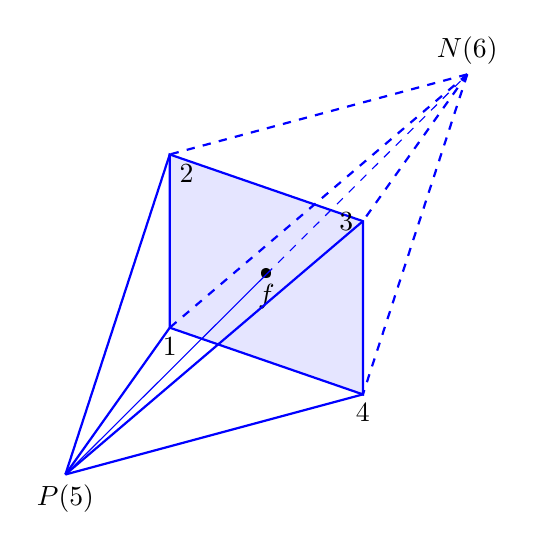
\begin{tikzpicture}[scale=1.1, every node/.style={scale=1}]
      
       %FACE DRAW
        \filldraw[color=blue,fill opacity=0.1,thick] (1.5,0,1)--(-1.5,0,-1)--(-1.5,2,-1)--(1.5,2,1)--cycle;
        %\draw[style=dashed,color=blue] (1.5,0,1)--(-1.5,2,-1);
        %\draw[style=dashed,color=blue] (1.5,2,1)--(-1.5,0,-1);
        \node at (0,1,0) {\textbullet};
        \draw (0,1,0) node[below] {$f$};
        
        \draw  (1.5,0,1) node[below] {$4$};
        \draw  (-1.5,0,-1) node[below] {$1$};
        \draw  (-1.5,2,-1) node[below right] {$2$};
        \draw  (1.5,2,1) node[left] {$3$};

        \draw [color=blue] (0,1,0)--(-0.01,1,6);
        \draw [color=blue,dashed] (0,1,0)--(0.01,1,-6);
        \draw  (-0.01,1,6) node[below] {$P(5)$};
        \draw  (0.01,1,-6) node[above] {$N(6)$};
        
        \draw [color=blue,thick] (-0.01,1,6)--(1.5,0,1);
        \draw [color=blue,thick] (-0.01,1,6)--(-1.5,0,-1);
        \draw [color=blue,thick] (-0.01,1,6)--(-1.5,2,-1);
        \draw [color=blue,thick] (-0.01,1,6)--(1.5,2,1);
        
        \draw [color=blue,thick,dashed] (0.01,1,-6)--(1.5,0,1);
        \draw [color=blue,thick,dashed] (0.01,1,-6)--(-1.5,0,-1);
        \draw [color=blue,thick,dashed] (0.01,1,-6)--(-1.5,2,-1);
        \draw [color=blue,thick,dashed] (0.01,1,-6)--(1.5,2,1);
        
      \end{tikzpicture}
    \caption{Геометрическая схема шаблона для численного нахождения частной производной на поверхности конечного объема $f$: $P$ обозначает центр ячейки с нормалью к $f$, $N$  обозначает центр ячейки, нормаль которой направлена внутрь конечного объема}
    \label{fig:derOnFace}
\end{figure}

Аппроксимация регуляризационных членов или, другими словами, $\tau$-слагаемых требует вычисления частных производных в центрах граней $f$, поскольку в выражениях потоков используются дифференциальные операторы градиента, дивергенции и их комбинации. В то время как нормальный к поверхности граней расчетных ячеек компонент дифференциальных операторов может быть аппроксимирован с помощью линейной интерполяции значений в центрах смежных с гранями ячеек, тангенциальные компоненты требуют особого подхода. Рассмотрены несколько подходов к аппроксимации $\tau$-слагаемых:
\begin{enumerate}
    \item вычисление с помощью центров ячеек использую линейную интерполяцию;
    \item метод пониженного порядка, предполагающий использование только нормальных компонентов производных, в то время как тангенциальными компонентами пренебрегается \cite{Kraposhin2017};
    \item метод наименьших квадратов \cite{Kraposhin2017};
    \item Метод Гаусса к фиктивному контрольному объему, определенному вокруг рассматриваемой грани $f$ \cite{Istomina2019}. В рамках этого метода расчетный шаблон включает вершины грани и точки в ячейках, прилегающих к грани (см рис. \ref{fig:derOnFace}). Например, выражение для $x$-производной скалярного поля $\alpha$ на четырехугольной грани имеет следующий вид::
    \begin{equation}
        \frac{\partial \alpha}{\partial x} \approx
        \frac{1}{V_f} \sum_{m=1}^8 n_{m,x} \alpha_m,
    \end{equation}
    где $V_f$ это объем фиктивной ячейки ограниченной поверхностями $f$, $m$ это индекс грани этой ячейки, $\alpha_m$ среднее значение $\alpha$ по грани $m$, $n_{m,x}$ это  $x$-компонент нормали к грани $m$.
    
\end{enumerate}

Наконец, дискретный аналог исходной системы состоит из:

\begin{itemize}
     \item дискретное алгебраическое уравнение (\ref{eq:qhd_approx_momentum}) для скорости $\vec U$, соответствующее уравнению импульса (\ref{eq:qhd_momentum});
     \item алгебраическое уравнение переноса (\ref{eq:qhd_approx_stransport}) для скаляра $s$, соответствующего уравнению (\ref{eq:qhd_stransport});
     \item выражение для регуляризованной скорости $\vec W^n $ (\ref{eq:qhd_approx_W});
     \item алгебраическое уравнение Пуассона для возмущения давления ~ (\ref{eq:qhd_approx_pressure}), соответствующее уравнению давления (\ref{eq:qhd_pressure}).
\end{itemize}

\begin{multline}\label{eq:qhd_approx_momentum}
    \frac{\delta \vec{U}}{\delta t} + \frac{1}{V} \sum_f \vec{S}_f \cdot \left( \vec{U}^o - \vec{W}^n \right)_f \otimes \vec{U}^o_f  - \frac{1}{V} \sum_f \nu_f \frac{\delta\vec{U}^n}{\delta \vec{n}_f} |\vec{S}_f| - \frac{1}{V} \sum_f \nu_f \vec{S}_f \cdot [\nabla \vec U^o]_f^T \\
    - \frac{1}{V} \sum_f \vec{S}_f \cdot \left( \vec{U}^o \otimes \vec{W}^n \right)_f = - \frac{1}{\rho_0} \frac{1}{V} \sum_f \tilde p^n_f \vec S_f + \vec{F}^o,
\end{multline}

\begin{multline}\label{eq:qhd_approx_stransport}
    \frac{\delta s}{\delta t} + \frac{1}{V}\sum_f \vec{S}_f \cdot \left (\vec{U}^o - \vec{W}^n \right)_f s^o_f - \frac{1}{V} \sum_f \frac{\nu_f}{Sc} \frac{\delta s^n}{\delta \vec{n_f}} |\vec{S}_f| - \\
    - \frac{1}{V} \sum_f \vec{S}_f \cdot \left( \tau_f \vec{U}_f  (\vec{U}_f \cdot [\nabla s^o]_f) \right) = 0,
\end{multline}

\begin{equation}\label{eq:qhd_approx_W}
    \vec W^n_f = \tau_f \left ( \vec U^o_f \cdot [\nabla \vec U^o]_f + \frac{1}{\rho_0} [\nabla \Tilde{p}^n]_f - \vec F^o_f  \right ),
\end{equation}

\begin{equation}\label{eq:qhd_approx_pressure}
        \frac{1}{V} \sum_f \frac{\tau_f}{\rho_0} \frac{\delta \tilde p^n}{\delta \vec{n_f}} |\vec{S}_f|  = \frac{1}{V} \sum_f \vec{S}_f \cdot \left( \vec{U}^o_f - \tau_f (\vec{U}^o_f \cdot [\nabla \vec{U}^o]_f ) + \tau_f \vec{F}^o_f \right),
\end{equation}
где $\frac{\delta}{\delta t}$ обозначает аппроксимацию производных по времени (например, Эйлера или Адамса-Башфорта), $\frac{\delta}{\delta \vec{n_f}} $ обозначает аппроксимацию производных по нормали к поверхности и квадратные скобки $[\cdot]_f$ обозначают аппроксимацию значения на грань $f$, которое может быть выполнено любым упомянутым ранее методом (приведенным, методом наименьших квадратов и т.д.).

Оценка значения $\tau$ (как среднего времени свободного пробега или характерного гидродинамического времени в случае жидкостей) дает диапазон от $\sim 10^{-10}$ c, для воздуха в атмосферных условиях до $\sim 10^{-13}$ c для воды в аналогичных условиях, что делает теоретическое определение $\tau$ непрактичным для реальных задач численного моделирования. Однако параметр регуляризации $\tau $ можно рассматривать как настраивающий коэффициент численной модели, которая вводит дополнительную управляемую диссипацию и гасит численные колебания и нестабильности. В этом случае значение $\tau $ может быть определено характерным временем: $\sim \nu / (\vec U \cdot \vec U) $ или в безразмерной форме с использованием чисел Рейнольдса и Грасгофа. Некоторые соображения по выбору $\tau$ для сжимаемых течений приведены в \cite{Kraposhin2018}.

Для несжимаемой жидкости определение $\tau$ включает в себя несколько шагов:

\begin{enumerate}
     \item Сделать приблизительную оценку, например, используя выражение $\tau = \frac{\nu}{\vec{U} \cdot \vec{U}}$ и соотношение $ \tau \sim Re^{-1} $ или $ \tau \sim Gr^{-1} $ и т.д.;
     \item Выполнть первое вычисление с заданным временным шагом и пространственным разрешением сетки и убедитесь, что решение гладкое. Если нет, то увеличьте значение $\tau $.
     \item Постепенно уменьшать $\tau$, чтобы проверить сходимость численного алгоритма (уточнение и исследование чувствительности).
\end{enumerate} 

\subsection{Реализация}

Алгебраические аналоги дифференциальных уравнений были реализованны на базе математического пакета с открытым исходным кодом OpenFOAM \cite{OpenFOAM}. Это набор средств для операций с полями, который включает в себя структуры данных для гидродинамических полей, эффективные инструменты для параллелизации, утилиты для решения алгебраических уравнений и средства выражения дифференциальных уравнений в частных производных на языке C++. 

Процедура реализации заключалось в разработке собственной программы-решателя квазигидродинамических уравнений. Ранее на базе openFOAM реализовывалась только классическая система уравнений Навье-Стокса \cite{PericCFDLecture}. 

Уже по алгоритму решения системы уравнений (рис. \ref{fig:blockSchemeQHD}) видно насколько он проще чем PISO. 

\begin{figure}
    \tikzstyle{decision} = [diamond, draw, 
    text width=4.5em, text badly centered, node distance=3cm, inner sep=0pt]
    \tikzstyle{block} = [rectangle, draw, 
    text width=30em, text centered, minimum height=3em, minimum width=30em]
    \tikzstyle{line} = [draw, -latex']
    \tikzstyle{cloud} = [draw, ellipse,fill=red!20, node distance=3cm,
    minimum height=2em]
    \centering
    \begin{tikzpicture}[node distance = 2cm, auto]
    % Place nodes
    	\node [block] (Start) {Начало};
        \node [block, below of=Start] (UpdateFl) {Вычисление потоков (1)};
        \node [block, below of=UpdateFl] (Pressure) {Решение уравнения давления (2)};
        \node [block, below of=Pressure] (Velocity) {Решение уравнения движения (3)};
        \node [block, below of=Velocity] (Salinity) {Решение уравнения переноса (4)};
        \node [block, below of=Salinity] (End) {Конец};

		\path [line] (Start) -- (UpdateFl);
        \path [line] (UpdateFl) -- (Pressure);
        \path [line] (Pressure) -- (Velocity);
        \path [line] (Velocity) -- (Salinity);
        \path [line] (Salinity) -- (End);
    \end{tikzpicture}   
    \caption{Блок-схема QHD алгоритма}
    \label{fig:blockSchemeQHD}
\end{figure}

\definecolor{codegreen}{rgb}{0,0.6,0}
\definecolor{codegray}{rgb}{0.5,0.5,0.5}
\definecolor{codepurple}{rgb}{0.58,0,0.82}
\definecolor{backcolour}{rgb}{0.95,0.95,0.92}

\lstdefinestyle{mystyle}{
    backgroundcolor=\color{backcolour},   
    commentstyle=\color{codegreen},
    keywordstyle=\color{magenta},
    numberstyle=\tiny\color{codegray},
    stringstyle=\color{codepurple},
    basicstyle=\ttfamily\footnotesize,
    breakatwhitespace=false,         
    breaklines=true,                 
    captionpos=b,                    
    keepspaces=true,                 
    numbers=left,                    
    numbersep=5pt,                  
    showspaces=false,                
    showstringspaces=false,
    showtabs=false,                  
    tabsize=2
}

\lstset{style=mystyle}

Перед началом расчета создаются основные поля в центрах ячеек, реализация приведена на рисунке \ref{fig:fieldsC}. Реализация использует типы данных математического пакета, такие как \verb|volScalarField| или \verb|volVectorField|, которые используются для скалярных и векторных полей соответственно.


\begin{figure}
    \centering
    \begin{lstlisting}
        volScalarField rho
        (
            IOobject
            (
                "rho",
                runTime.timeName(),
                mesh,
                IOobject::NO_READ,
                IOobject::AUTO_WRITE
            ),
            thermo.rho()
        );
        
        volVectorField W
        (
            IOobject
            (
                "W",
                runTime.timeName(),
                mesh,
                IOobject::NO_READ,
                IOobject::NO_WRITE
            ),
            U
        );
    \end{lstlisting}
    \caption{Пример выделения памяти для гидродинамических полей в центрах расчетных ячеек в терминах openFOAM}
    \label{fig:fieldsC}
\end{figure}

Затем вычисляются гидродинамические поля на гранях расчетных ячеек (\ref{fig:fieldsF}), для этого используется линейная интерполяция с центров двух соседних ячеек с помощью функции \verb|linearInterpolate|.

\begin{figure}
    \centering
    \begin{lstlisting}
        // Density
        surfaceScalarField rhof
        (
            "rhof",
            linearInterpolate(rho)
        );
    
        // Velocity
        surfaceVectorField Uf
        (
            "Uf",
            linearInterpolate(U)
        );
    
        // Additional velocity
        surfaceVectorField Wf
        (
            "Wf",
            linearInterpolate(W)
        );
    \end{lstlisting}
    \caption{Пример выделения памяти для гидродинамических полей на гранях в терминах openFOAM}
    \label{fig:fieldsF}
\end{figure}

После этого вычисляются производные на гранях вычислительных ячеек (рис. \ref{fig:fieldsFD}). 

\begin{figure}
    \centering
    \begin{lstlisting}
    surfaceVectorField gradPf
    (
        "gradPf", fvsc::grad(p)
    );

    surfaceTensorField gradUf
    (
        "gradUf",
        fvsc::grad(U)
    );

    surfaceTensorField gradWf
    (
        "gradWf",
        fvsc::grad(W)
    );

    surfaceVectorField gradTf
    (
        "gradTf",
        fvsc::grad(T)
    );
    \end{lstlisting}
    \caption{Пример вычисления производных на гранях вычислительных ячеек.}
    \label{fig:fieldsFD}
\end{figure}

Вычисления производных на гранях регулируется пользователем, имеется возможность выбрать одну из схем перечисленных выше.

\begin{figure}
    \centering
    
\begin{lstlisting}

    fvsc
    {
        default    GaussVolPoint;
    }

\end{lstlisting}

    \caption{Интерфейс управления схемой вычисления производных на гранях вычислительного объема.}
    \label{fig:fvscList}
\end{figure}

Затем начинается вычислительный цикл изображенный на рисунке \ref{fig:blockSchemeQHD}. В ходе этого цикла вычисляются потоки (рис. \ref{fig:fluxes}).

\begin{figure}
    \centering
    \begin{lstlisting}
    phiu  = mesh.Sf() & Uf;
    phiu.setOriented(true);
    
    phiwo = mesh.Sf() & (tauQGDf*((Uf & gradUf) - BdFrcf));
    phiwo.setOriented(true);
    
    taubyrhof = tauQGDf/rhof;
    \end{lstlisting}
    \caption{Пример вычисления производных на гранях вычислительных ячеек.}
    \label{fig:fluxes}
\end{figure}

Потом решается уравнение для давления (рис. \ref{fig:peqn}).

\begin{figure}
    \centering
    \begin{lstlisting}
    
    //Continuity equation
    p.correctBoundaryConditions();
    fvScalarMatrix pEqn
    (
         fvc::div(phiu)
        -fvc::div(phiwo)
        -fvm::laplacian(taubyrhof,p)
    );
    
    pEqn.setReference(pRefCell, getRefCellValue(p, pRefCell));
    
    pEqn.solve();
    
    phi = phiu - phiwo + pEqn.flux();
    
    \end{lstlisting}
\caption{Решение уравнения для давления в терминах openFOAM}
\label{fig:peqn}
\end{figure}

После этого решается уравнение баланса импульса (рис. \ref{fig:velList})

\begin{figure}
\centering
\begin{lstlisting}
    gradPf = fvsc::grad(p);
    Wf = tauQGDf*((Uf & gradUf) + gradPf/rhof - BdFrcf);
    surfaceVectorField phiUfWf = mesh.Sf() & (Uf * Wf);
    phiUf -= phiUfWf;

    {
    solve
        (
            fvm::ddt(U)
            +
            fvc::div(phiUf)
            -
            fvm::laplacian(muf/rhof,U)
            -
            fvc::div(muf/rhof * mesh.Sf() 
            & qgdInterpolate(Foam::T(fvc::grad(U))))
            ==
            -
            fvc::grad(p)/rho
            +
            BdFrc
            +
            USu
        );
    }
\end{lstlisting}
\caption{Решение уравнения баланса импульса в терминах openFOAM}
\label{fig:velList}
\end{figure}

И наконец решается уравнение переноса (рис. \ref{fig:trans}).


\begin{figure}
    \centering
\begin{lstlisting}
if (implicitDiffusion)
{
    solve(fvm::ddt(T) - fvc::ddt(T) - fvm::laplacian(Hif, T) == TSu);
}
else
{
    solve(fvm::ddt(T) - fvc::ddt(T) - fvc::laplacian(Hif, T) == TSu);
}
\end{lstlisting}    
\caption{Решение уравнения переноса в терминах openFOAM}
\label{fig:trans}
\end{figure}

Также есть возможность управления параметром регуляризации:

\begin{figure}
    \centering
\begin{lstlisting}

    QGD
    {
        pRefCell        0;
        pRefValue       0;
        implicitDiffusion true;
        QGDCoeffs constTau;
        constTauDict
        {
            Tau 0.005;
        }
    }

\end{lstlisting}    
    \caption{Часть файла управления вычислением $\tau$-слагаемыми.}
    \label{fig:QGD}
\end{figure}

\subsection{Верификация}

QHDSolver это программа для моделирования движения несжимаемой жидкости. Важным свойством таких программ является чувствительность к физическим параметрам, таким как скорость, плотность, вязкость и размеры расчетной области. Эти параметры объеденяются в число рейнольдса. Также необходимо найти корректное решения для уравнения переноса. QHDSolver позиционируется как программа призванная работать с неортогональными сетками и находить корректное решение. Для демонстрации возможности решателя было выбрано несколько типовых задач. Для верификации возможности работы с неортогональными сетками была выбрана задача скошенной каверны. Чувствительность к числу Рейнольдса проверяется на задаче обратного уступа. Корректность решения уравнения переноса проверяется на задаче естественной конвекции. Полученные результаты сравниваются с результатами других исследователей.

\paragraph{Скошенная каверна}

Квазигидродинамический решатель сравнивается с PISO алгоритмом на метках низкого качества. Главной целью этого сравнения является демонстрация возможностей программы корректно решать задачи поставленные на неортогональных сетках и сложных геометриях. Эксперимент определяется следующими настроечными параметрами:

\begin{itemize}
    \item Размер сетки
    \item Шаг по времени
    \item Параметр регуляризации
    \item Число Рейнольдса
    \item Угол скошенности ($\alpha$)
\end{itemize}

Моделирование исследует сеточную сходимость при числах рейнольдса 100 и 1000, углах скошенности $\alpha = \{45^{\circ}, 30^{\circ}, 15^{\circ}$\}. Схематично рассчетная область изображена на рисунке \ref{fig:skewedCavityScratch}. На верхней границе задана постоянная скорость $\vec{U}_b$ и нулевой градиент для давления. На других стенках установлено условие нулевой скорости и градиента давления.

\begin{figure}
    \centering
    \begin{tikzpicture}[scale=6, every node/.style={scale=1}]
            \draw (0,0,0)--(1,0,0)--(1.7071,0.7071,0.0)--(0.7071,0.7071,0.0)--cycle;
            \draw [color=blue] (0.5,0,0)--(1.2071,0.7071,0);
            
            \draw [->,>=stealth](0.7071,0.735,0.0)-- (1.7071,0.735,0.0);
            \draw  (1.2071,0.72,0) node[above] {$\vec{U}_b$};
            
            \draw  (0.5,0,0) node[below] {$B$};
            \draw  (1.2071,0.7071,0) node[below] {$A$};

            \draw (0.15,0) arc (0:65:1mm);
            \draw (0.18,0.04,0) node[above] {$\alpha$};
            
    \end{tikzpicture}
    \caption{Схематичное представление верификационной задачи с косоугольной каверной, вдоль линии AB ведутся замеры горизонтальной компоненты скорости.}
    \label{fig:skewedCavityScratch}
\end{figure}

Компоненты поля скорости, полученные с помощью QHDFoam сравниваются с теми же компонентами полученными при помощи pimpleFOAM. Рассматривается зависимость решения от параметра регуляризации и шага по времени. Результаты моделирования также сравниваются с результатами полученными ранее другими исследователями \cite{Hines2008,Erturk2007}. 

Сравнение QHD и PIMPLE алгоритмом с числами рейнольдса $Re=100$ и $Re=1000$ $\alpha = 45^{\circ}$, $\alpha = 30^{\circ}$ демонстрируют схожесть результатов (см рис. \ref{fig:Re10045UxVSy} - \ref{fig:15UxVSYRe100}). Сетки с элементами более чем 20х20 дают отличное соотвествие с эталонным решением \cite{Erturk2007}. Для случаев с маленькими углами скошенности и числами Рейнольдса алгоритмы типа PISO не могут найти решение без коррекций на неортогональность. QHDFoam могут быть применены без дополнительных коррекций, для этого требуется увеличить параметр регуляризации или уменьшить шаг по времени.

Каждая конфигурация каверны исследована на сеточную сходимость. Обычно сетки более 40х40 элементов дают точность с ошибкой не более 5\%. Более подробные сетки дают точность с ошибкой меньше чем 3\%. Результаты сеточной сходимости приведены на рисунке \ref{fig:meshconv}, он показывает порядок метода между теоретическими линиями соответствующих первому и второму порядку.

Разность результатов полученных при помощи квазигидродинамического подхода и при помощи PISO представленная на рисунках \ref{fig:15UxVSYRe100} -- \ref{fig:r15} может быть объяснена дополнительной диссипацией, которая привносится квазигидродинамическим алгоритмом. Очевидно, что ошибка тем меньше чем, меньше параметр регуляризации. Начальное значение для этого параметра может быть выбрано согласно значению числа Рейнольдса и условию устойчивости:

\begin{equation}
    \Delta t \leq c \cdot \tau,
\end{equation}

Где $\Delta t$ это шаг по времени, $\tau$ это регуляризационный параметр, коэффициент $c$ зависит от скошенности. Опытным путем установлено что для $\alpha = 90^{\circ}$ $c=2$, но для $\alpha = 15^{\circ}$ $c=24$.

Для увеличения точности PISO алгоритма на неортогональных сетках требуется увеличивать сеточное разрешения и количество коррекций на неортогональность. Для увеличения точности квазигидродинамического алгоритма кроме увеличения количества ячеек необходимо уменьшить шаг по времени и параметр регуляризации согласно условию устойчивости (см. рис. \ref{fig:tauconv}). 

\begin{figure}[!ht]
    \centering
        \begin{tikzpicture}[scale = 1.2]
        
            \begin{axis}
                [scale only axis, grid=major, ymin=0, ymax=0.75, xmax = 1, xmin = -0.2, legend style={at={(1,0.71)},anchor=north east},legend style={nodes={scale=1, transform shape}},xlabel={$y$}, ylabel={$U_x$}]
                \addplot[solid,thick, color=red] table [y=Points:1, x=U:0, col sep=comma]     {PISOVSQHD/PISOUxVSY100Re20.csv};
                \addplot[solid,thick, color=orange] table [y=Points:1, x=U:0, col sep=comma]     {PISOVSQHD/PISOUxVSY100Re40.csv};

                \addplot[solid,thick, color=green] table [y=Points:1, x=U:0, col sep=comma]     {PISOVSQHD/QHDUxVSY100Re20.csv};
                \addplot[solid,thick, color=cyan] table [y=Points:1, x=U:0, col sep=comma]     {PISOVSQHD/QHDUxVSY100Re40.csv};
                \addplot[solid,thick, color=blue] table [y=Points:1, x=U:0, col sep=comma]     {PISOVSQHD/QHDUxVSY100Re80.csv};
                \addplot[solid,thick, color=black] table [y=Y, x=Ux, col sep=comma]     {PISOVSQHD/Eth45Re100.csv};
                \legend{PISO 20x20, PISO 40x40, QHD 20x20, QHD 40x40, QHD 80x80, Eth}
            \end{axis}
        
        \end{tikzpicture}
        \caption{Re=100, $\alpha = 45^\circ$, зависимость $U_x$ от $y$, скорость вдоль линии AB.}
        \label{fig:Re10045UxVSy}
\end{figure}

\begin{figure}[!ht]
    \centering
        \begin{tikzpicture}[scale = 1.2]
        
            \begin{axis}
                [scale only axis, grid=major, ymin=0, ymax=0.525, xmax = 1, xmin = -0.2, legend style={at={(1,0.5)},anchor=north east},legend style={nodes={scale=0.8, transform shape}},xlabel={$U_x$}, ylabel={$y$}]
                \addplot[solid,thick, color=red] table [y=Points:1, x=U:0, col sep=comma]     {PISOVSQHD/PISO30UxVSY1000Re20.csv};
                \addplot[solid,thick, color=orange] table [y=Points:1, x=U:0, col sep=comma]     {PISOVSQHD/PISO30UxVSY1000Re40.csv};
                \addplot[solid,thick, color=yellow] table [y=y, x=U_0, col sep=comma]     {PISOVSQHD/PISOCor30UxVSY1000Re80.csv};
                \addplot[solid,thick, color=green] table [y=Points:1, x=U:0, col sep=comma]     {PISOVSQHD/QHD30UxVSY1000Re20.csv};
                \addplot[solid,thick, color=cyan] table [y=Points:1, x=U:0, col sep=comma]     {PISOVSQHD/QHD30UxVSY1000Re40.csv};
                \addplot[solid,thick, color=blue] table [y=Points:1, x=U:0, col sep=comma]     {PISOVSQHD/QHD30UxVSY1000Re80.csv};
                \addplot[only marks, color=black] table [y=Y, x=Ux, col sep=comma]     {PISOVSQHD/Eth30UxVSYRe1000.csv};
                \legend{PISO 20x20, PISO 40x40,  PISO 80x80*, QHD 20x20, QHD 40x40, QHD 80x80, Eth}
            \end{axis}
        
        \end{tikzpicture}
        \caption{Re=1000, $\alpha = 30^\circ$, зависимость $U_x$ от $y$, горизонтальная компонента сокрости вдоль линии AB.}
        \label{fig:30UxVSY1000Re}
\end{figure}


\begin{figure}[!ht]
    \centering
        \begin{tikzpicture}[scale = 1.25]
            \begin{axis}[scale only axis, grid=major, ymin=-2.2*10^-2, ymax=2*10^-2, xmin = 0.42, xmax = 1.45, legend style={at={(0.4,1)},anchor=north east},legend style={nodes={scale=0.8, transform shape}},xlabel={$x$}, ylabel={$U_y$}]

                \addplot[solid,thick, color=red] table [x=Points:0, y=U:1, col sep=comma]     {PISOVSQHD/PISO30UyVSX1000Re20.csv};
                \addplot[solid,thick, color=orange] table [x=Points:0, y=U:1, col sep=comma]     {PISOVSQHD/PISO30UyVSX1000Re40.csv};
                \addplot[solid,thick, color=yellow] table [x=x, y=U_1, col sep=comma]     {PISOVSQHD/PISOCor30UyVSX1000Re80.csv};
                \addplot[solid,thick, color=green] table [x=Points:0, y=U:1, col sep=comma]     {PISOVSQHD/QHD30UyVSX1000Re20.csv};
                \addplot[solid,thick, color=cyan] table [x=Points:0, y=U:1, col sep=comma]     {PISOVSQHD/QHD30UyVSX1000Re40.csv};
                \addplot[solid,thick, color=blue] table [x=Points:0, y=U:1, col sep=comma]     {PISOVSQHD/QHD30UyVSX1000Re80.csv};
                \addplot[only marks, color=black] table [x=X, y=Uy, col sep=comma]     {PISOVSQHD/Eth30UyVSXRe1000.csv};
                \legend{PISO 20x20, PISO 40x40, PISO 80x80*, QHD 20x20, QHD 40x40, QHD 80x80, Eth}
            \end{axis}
         \end{tikzpicture}
         \caption{Re=1000, $\alpha = 30^\circ$, зависимость $U_y$ от $x$, вертикальная компонента скорости вдоль линии CD, звездочкой обозначен результат проведенный с помощью коррекций на неортогональность}
         \label{fig:30UyVSXRe1000}
\end{figure}


\begin{figure}[!ht]
     \centering
         \begin{tikzpicture}[scale = 1.25]
             \begin{axis}
             [scale only axis, grid=major, ymin=0, ymax=0.3, xmax = 1, xmin = -0.2, legend style={at={(1,0.71)},anchor=north east},legend style={nodes={scale=1, transform shape}},xlabel={$U_x$}, ylabel={$y$}]
                 \addplot[solid,thick, color=red] table [y=Points:1, x=U:0, col sep=comma] {PISOVSQHD/PISOCor15UxVSY100Re80.csv};
                 \addplot[solid,thick, color=green] table [y=Points:1, x=U:0, col sep=comma]     {PISOVSQHD/QHD15UxVSY100Re20.csv};
                 \addplot[solid,thick, color=cyan] table [y=Points:1, x=U:0, col sep=comma]     {PISOVSQHD/QHD15UxVSY100Re40.csv};
                 \addplot[solid,thick, color=blue] table [y=y, x=U_0, col sep=comma] {PISOVSQHD/UxVSY15Re100M80Tu5.csv};
                 \addplot[only marks, color=black] table [y=Y, x=Ux, col sep=comma]     {PISOVSQHD/Eth15UxVSYRe100.csv};
                 \legend{PISO 80x80*, QHD 20x20, QHD 40x40, QHD 80x80, Eth};
             \end{axis}
         \end{tikzpicture}
         \caption{Re=100, $\alpha = 15^\circ$, зависимость $U_x$ от $y$, горизонтальная компонента скорости вдоль линии AB, звездочкой обозначены результаты полученный с использованием поправок на неортогональность}
         \label{fig:15UxVSYRe100}
\end{figure}

\begin{figure}[!ht]
    \centering
        \begin{tikzpicture}[scale = 1.2]
            \begin{axis}[scale only axis, grid=major, ymin=-8.2*10^-2, ymax=12*10^-2, xmin = 0.5, xmax = 1.5, legend style={at={(0.5,0.36)},anchor=north east},legend style={nodes={scale=0.8, transform shape}},xlabel={$x$}, ylabel={$U_y$}]
                \addplot[solid,thick, color=red] table [x=Points:0, y=U:1, col sep=comma]     {PISOVSQHD/PISOCor15UyVSX100Re80.csv};
                \addplot[solid,thick, color=green] table [x=Points:0, y=U:1, col sep=comma]     {PISOVSQHD/QHD15UyVSX100Re20.csv};
                \addplot[solid,thick, color=cyan] table [x=Points:0, y=U:1, col sep=comma]     {PISOVSQHD/QHD15UyVSX100Re40.csv};
                \addplot[solid,thick, color=blue] table [x=x, y=U_1, col sep=comma] {PISOVSQHD/UyVSX15Re100M80Tu5.csv};
                \addplot[only marks, color=black] table [y=Uy, x=x, col sep=comma]     {PISOVSQHD/Eth15UyVSXRe100.csv};
                \legend{PISO 80x80*, QHD 20x20, QHD 40x40, QHD 80x80, Eth};
            \end{axis}
        \end{tikzpicture}
        \caption{Re=100, $\alpha = 15^\circ$, зависимость $U_y$ от $x$, вертикальная компонента скорости вдоль линии AB, звездочкой обозначены результаты полученные с использованием поправок на неортогональность}
        \label{fig:15UyVSXRe100}
\end{figure}

 \begin{figure}[!ht]
     \centering
         \begin{tikzpicture}[scale = 1.2]
            \begin{axis}
                [scale only axis, grid=major, ymin=-4.8*10^-2, ymax=3*10^-2, xmin = 0.47, xmax = 1.5, legend style={at={(0.5,0.5)},anchor=north east},legend style={nodes={scale=0.6, transform shape}},xlabel={$x$}, ylabel={$U_y$}]
                \addplot[solid,thick, color=red] table [x=Points:0, y=U:1, col sep=comma]     {PISOVSQHD/QHD15UyVSX1000Re512.csv};
                \addplot[only marks, color=black] table [x=X, y=Uy, col sep=comma]     {PISOVSQHD/Eth15UyVSXRe1000.csv};
                \addplot[solid,thick, color=blue] table [x=Points:0, y=U:1, col sep=comma]     {PISOVSQHD/QHD15UyVSX1000Re80Tu24.csv};
                \addplot[solid,thick, color=cyan] table [x=Points:0, y=U:1, col sep=comma]     {PISOVSQHD/QHD15UyVSX1000Re80Tu10.csv};
                 \addplot[solid,thick, color=gray] table [x=Points:0, y=U:1, col sep=comma]     {PISOVSQHD/QHD15UyVSX1000Re80Tu5.csv};
                \legend{QHD 512x512, Eth, QHD 80x80 $\tau = 0.024$, QHD 80x80 $\tau = 0.010$, QHD 80x80 $\tau = 0.005$};
            \end{axis}
         \end{tikzpicture}
         \caption{Re=1000, $\alpha = 15^\circ$, зависимость $U_y$ от $x$, влияние параметра регуляризации на решение.}
         \label{fig:r15}
 \end{figure}

\begin{figure}[!ht]
    \centering
        \begin{tikzpicture}[scale = 1.2]
            \begin{axis}
                [scale only axis, grid=major, ymin=-4.8*10^-2, ymax=3*10^-2, xmin = 0.47, xmax = 1.5, legend style={at={(0.6,0.5)},anchor=north east},legend style={nodes={scale=0.8, transform shape}},xlabel={$x$}, ylabel={$U_y$}]
                \addplot[solid,thick, color=red] table [x=Points:0, y=U:1, col sep=comma]     {PISOVSQHD/QHD15UyVSX1000Re512.csv};
                \addplot[only marks, color=black] table [x=X, y=Uy, col sep=comma]     {PISOVSQHD/Eth15UyVSXRe1000.csv};
                \addplot[solid,thick, color=blue] table [x=Points:0, y=U:1, col sep=comma]     {PISOVSQHD/QHD15UyVSX1000Re80Tu24.csv};
                \addplot[solid,thick, color=cyan] table [x=Points:0, y=U:1, col sep=comma]     {PISOVSQHD/QHD15UyVSX1000Re80Tu10.csv};
                 \addplot[solid,thick, color=gray] table [x=Points:0, y=U:1, col sep=comma]     {PISOVSQHD/QHD15UyVSX1000Re80Tu5.csv};
                \legend{QHD 512x512, Eth, QHD 80x80 $\tau = 0.024$, QHD 80x80 $\tau = 0.010$, QHD 80x80 $\tau = 0.005$};
            \end{axis}
        \end{tikzpicture}
        \caption{Re=1000, $\alpha = 15^\circ$, зависимость $U_y$ от $x$}
        \label{fig:tauconv}
\end{figure}

\begin{figure}[!ht]
    \centering
        \begin{tikzpicture}[scale = 1.5]
            \begin{axis}
                [ymode=log,xmode=log,xlabel={Количество ячеек}, ylabel={$L_1 error$}]
                \addplot[solid,thick, color=red] table [x=N, y=L1, col sep=comma]{PISOVSQHD/meshConv.csv};
                \addplot[solid,thick,dashed, color=blue] table [x=N, y=L1, col sep=comma]
                {PISOVSQHD/meshConvEth.csv};
                \addplot[solid,thick,dashed, color=green] table [x=N, y=L1, col sep=comma]{PISOVSQHD/meshConvEth1Ord.csv};
            \end{axis}
        \end{tikzpicture}
        \caption{Сеточная сходимость, порядок метода}
        \label{fig:meshconv}
\end{figure}

\begin{figure}
    \centering
        \begin{tikzpicture}[scale = 1.2]
            \begin{axis}
                [scale only axis, grid=major, ymin=-0.02, ymax=0.25, xmin = 0.0, xmax = 1.1, legend style={at={(0.45,0.9)},anchor=north east},legend style={nodes={scale=1, transform shape}}]
                \addplot[solid,thick, color=black] table [x=l, y=UyTau0.004, col sep=comma]     {CSV/AllTau.csv};
                \addplot[solid,thick, color=orange] table [x=l, y=UyTau0.005, col sep=comma]     {CSV/AllTau.csv};
                \addplot[solid,thick, color=green] table [x=l, y=UyTau0.01, col sep=comma]     {CSV/AllTau.csv};
                \addplot[solid,thick, color=cyan] table [x=l, y=UyTau0.02, col sep=comma]     {CSV/AllTau.csv};
                \addplot[solid,thick, color=gray] table [x=l, y=UyTau0.04, col sep=comma]     {CSV/AllTau.csv};
                \addplot[solid,thick, color=brown] table [x=l, y=UyTau0.08, col sep=comma]     {CSV/AllTau.csv};
                \addplot[solid,thick, color=red] table [x=l, y=UyTau0.16, col sep=comma]     {CSV/AllTau.csv};
                \legend{$\tau = 0.004$, $\tau = 0.005$, $\tau = 0.01$, $\tau = 0.02$, $\tau = 0.04$,$\tau = 0.08$,$\tau = 0.16$}
            \end{axis}
        \end{tikzpicture}
        \caption{Re=1000, $\alpha = 45^\circ$, $U_y$ vs $x$, влияние параметра регуляризации на решение}
\end{figure}

Рассчитанное гидродинамическое поле скорости для $\alpha = 30^{\circ}$ и $\alpha = 45^{\circ}$ показано на рисунке \ref{fig:SCav}.

\begin{figure}
    \centering
    \begin{subfigure}[b]{0.45\textwidth}
        \begin{tikzpicture}[scale=4.5, every node/.style={scale=1}]
            \node[anchor=south west,inner sep=0] at (0,0) {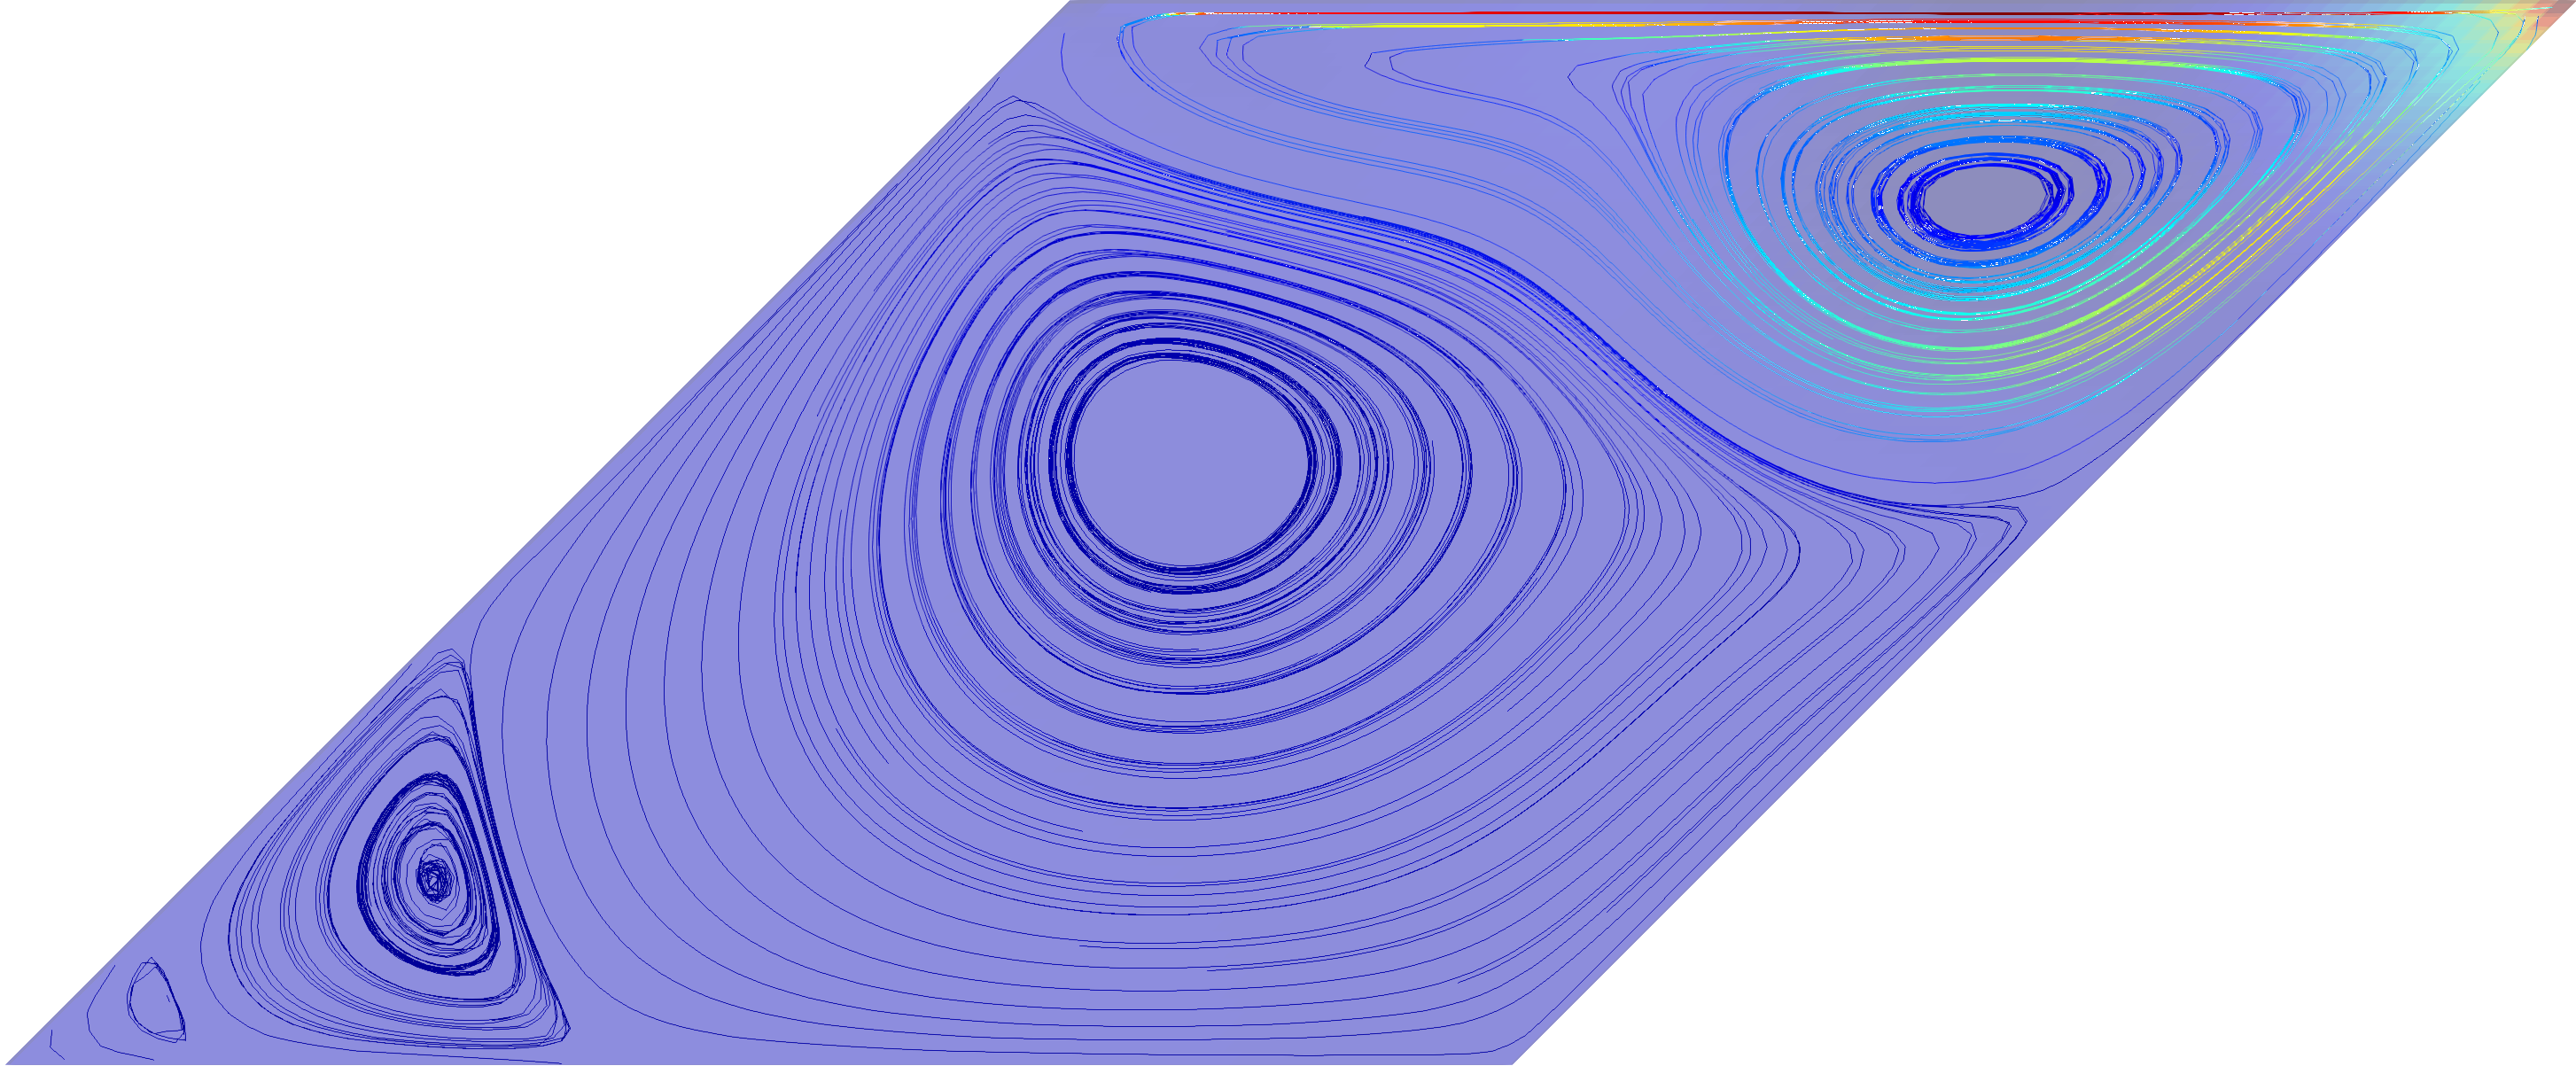
\includegraphics[width=1.055\textwidth]{pics/StreamlinesAtPressureCrop.png}};
            \draw (0,0,0)--(1,0,0)--(1.7071,0.7071,0.0)--(0.7071,0.7071,0.0)--cycle;
            \draw [color=black] (0.5,0,0)--(1.2071,0.7071,0);
            
            \draw [->,>=stealth](0.7071,0.735,0.0)-- (1.7071,0.735,0.0);
            \draw  (1.2071,0.72,0) node[above] {$\vec{U}_b$};
            
            \draw  (0.5,0,0) node[below] {$B$};
            \draw  (1.2071,0.7071,0) node[below] {$A$};

            \draw (0.15,0) arc (0:65:1mm);
            \draw (0.18,0.04,0) node[above] {$\alpha$};
        \end{tikzpicture}
        \caption{}
    \end{subfigure}
    \begin{subfigure}[b]{0.45\textwidth}
        \centering
        \begin{tikzpicture}[scale=4.5, every node/.style={scale=1}]
            \node[anchor=south west,inner sep=0] at (0,0) {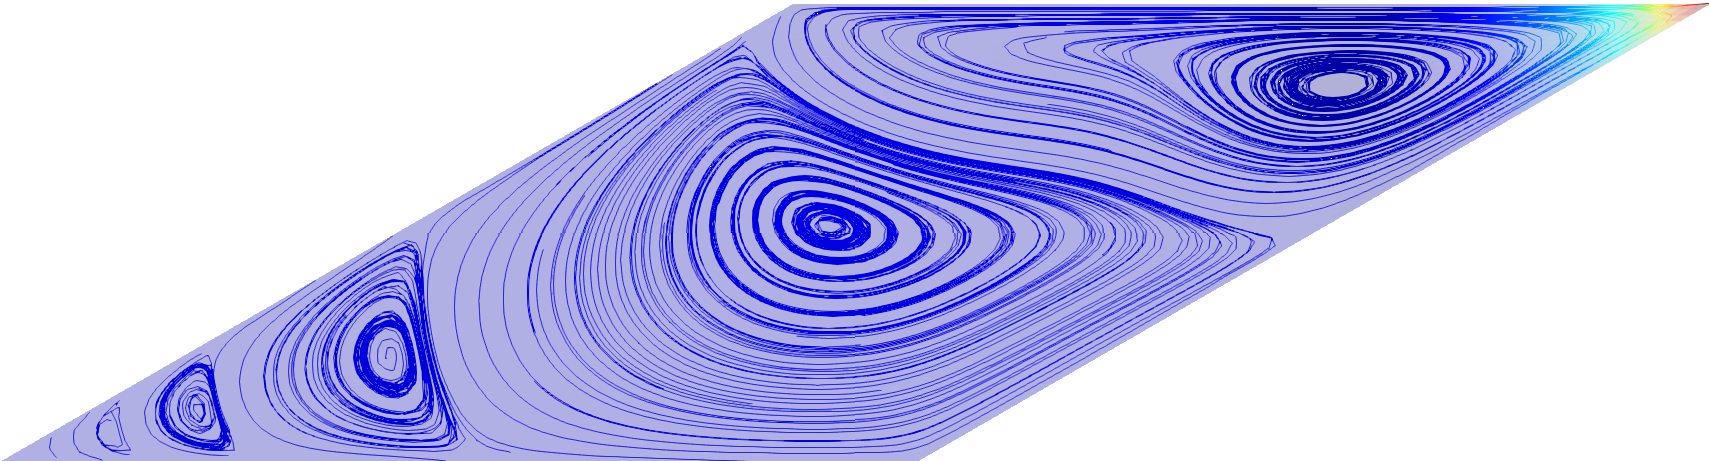
\includegraphics[width=1.15\textwidth]{pics/StreamlinesAtPressureCropTikz30.png}};
            \draw (0,0,0)--(1,0,0)--(1.86,0.5,0.0)--(0.86,0.5,0.0)--cycle;
            \draw [color=black] (0.5,0,0)--(1.36,0.5,0);
            
            \draw [->,>=stealth](0.86,0.523,0.0)-- (1.86,0.523,0.0);
            \draw  (1.35,0.52,0) node[above] {$\vec{U}_b$};
            
            \draw  (0.5,0,0) node[below] {$B$};
            \draw  (1.3071,0.5071,0) node[below] {$A$};

            \draw (0.21,0) arc (0:65:1mm);
            \draw (0.28,0.04,0) node[above] {$\alpha$};
            
        \end{tikzpicture}
        \caption{}
    \end{subfigure}
    \caption{Схематичное представление верификационной задачи с косоугольной каверной, горизонтальная компонента скорости замеряется вдоль линии AB.}
    \label{fig:SCav}
\end{figure}

\paragraph{Обратный уступ}

Для моделирования вязкой жидкости, алгоритму необходимо быть чувствительным к изменению числа Рейнольдса. Задача обратного уступа это простой и эффективный способ проверить эту чувствительность. На вход в расчетную область подается параболический профиль скорости. Все стенки кроме входа и выхода подчиняются условию прилипания для скорости и нулевого градиента для давления. 

После стабилизации потока измеряется расстояния от левой твердой стенки до точки разворота потока($d$) (см рис. \ref{fig:backwardStepSketch}). Полученное значение $d$ сравнивается с эталонным из \cite{ElizarBook}. Результаты показывают что QHDFoam корректно разрешает вязкие течения (см. рис. \ref{StreamRe100})

\begin{figure}[!h]
    \centering
    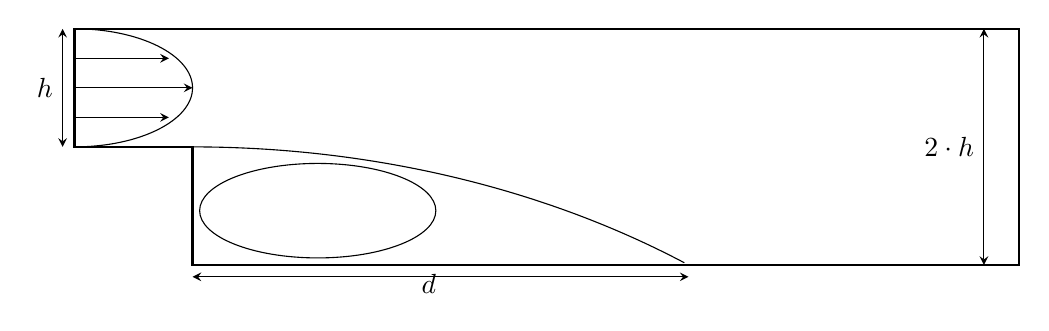
\begin{tikzpicture}[scale=1.5, every node/.style={scale=1}]
        \draw[thick] (0,2,0)--(0,1,0)--(1.0,1.0,0.0)--(1.0,0.0,0.0)--(8.0,0.0,0.0)--(8.0,2.0,0.0)--cycle;
            
        \draw (0.0,1.0) arc(-90:90:1cm and 0.5cm);
        \draw [->,>=stealth](0.0,1.5,0.0)-- (1,1.5,0.0);
        \draw [->,>=stealth](0.0,1.25,0.0)-- (0.8,1.25,0.0);
        \draw [->,>=stealth](0.0,1.75,0.0)-- (0.8,1.75,0.0);
        
        
        \draw (2.06,0.06) arc(-90:270:1cm and 0.4cm);
        \draw [<->,>=stealth](1,-0.1)--(5.2,-0.1);
        \draw (3,0.0,0) node[below] {$d$};
        
        \draw [<->,>=stealth](-0.1,1)--(-0.1,2);
        \draw (-0.1,1.5,0) node[left] {$h$};
        
        \draw [<->,>=stealth](7.7,0)--(7.7,2);
        \draw (7.7,1,0) node[left] {$2 \cdot h$};
        \draw (1.0,1.0) arc(90:53.5:7cm and 5cm);
    \end{tikzpicture}
    \caption{Схематичное изображение задачи с обратным уступом.}
    \label{fig:backwardStepSketch}
\end{figure}

\begin{figure}[!h]
    \centering
    \begin{subfigure}{\textwidth}
        \centering
        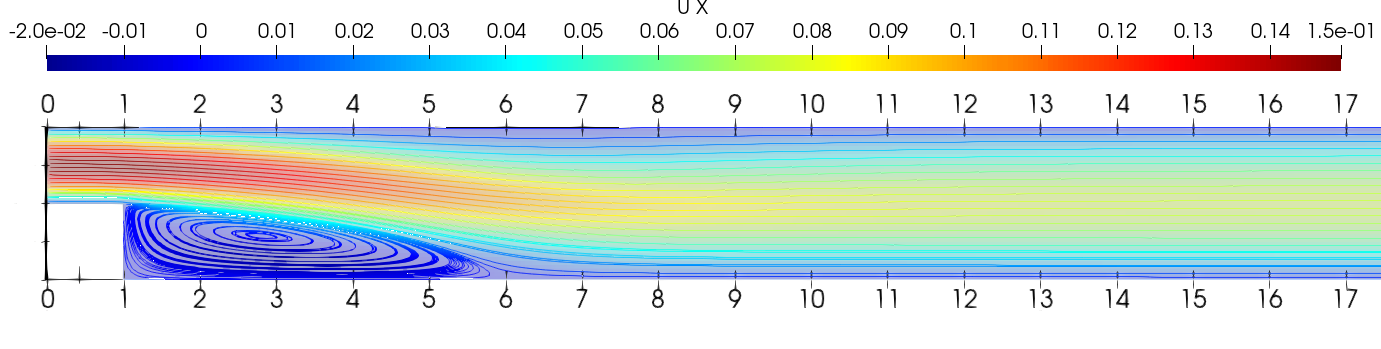
\includegraphics[scale=0.4]{pics/Re100.png}
        \caption{Re=100}
    \end{subfigure}
    \begin{subfigure}{\textwidth}
        \centering
        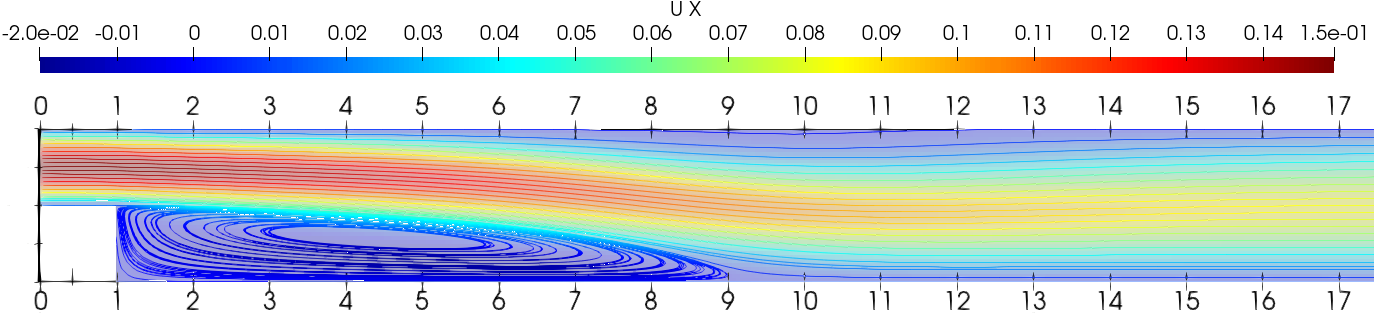
\includegraphics[scale=0.4]{pics/Re200.png}
        \caption{Re=200}
    \end{subfigure}
    \begin{subfigure}{\textwidth}
        \centering
        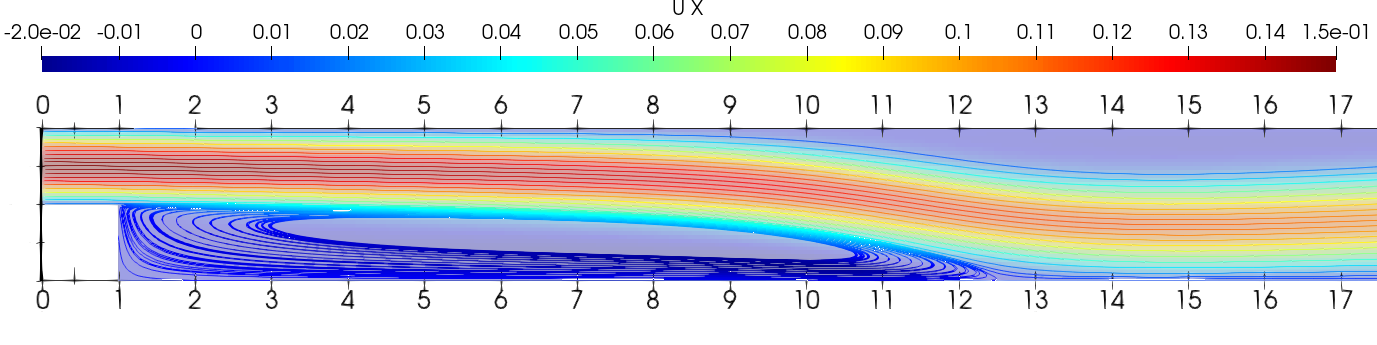
\includegraphics[scale=0.4]{pics/Re400.png}
        \caption{Re=400}
    \end{subfigure}
    \caption{Линии тока для задачи с обратным уступом}
    \label{StreamRe100}
\end{figure}


\begin{table}[!hb]
\caption {Сравнение результатов для задачи обратного уступа}
\noindent\begin{tabular}{l|ccc}
Research & $Re=100$ & $Re=200$  & $Re=400$ \\
\hline
QHDFoam & 5.0 & 8.25 & 11.9\\
Sparrow E. M. and Chuck W.\cite{Sparrow1987} & 5.0 & 7.5 & -\\
Kim J. and Moin P.\cite{Kim1985} & 5.0 & 8.3 & 12 \\
Hackman L. P. et al.\cite{Hackman1984} & 5.0 & 8.5 & -\\
\hline
Armaly B. F. et al.\cite{Armaly1983} & 5.0 & 8.5 & 14.2
\end{tabular}
\label{table:tabBackward}
\end{table}

\paragraph{Естественная конвекция}

Рассматривается задача естественной конвекции в каверне согласно \cite{ElizarBook} значение регуляризационного параметра было вычислено пропорционально обратному числу Грастгофа $Gr^{-1}$, которое было порядка $10^{-4}$ с. Сравнение максимумов горизонтальной и вертикальной скорости с данными из \cite{ElizarBook} и \cite{Vabishevich} показывают сеточную сходимость и хорошую согласованность между QHDFoam и рассматриваемыми в работах методами. Результаты сравнения видны в таблице \ref{table:tabHotCavityHor} . Линии тока изображены на рисунке \ref{fig:Nconv}. Схему расчетной области можно увидеть на рисунке \ref{fig:convectionScratch}

\begin{table}[!hb]
\caption { Сравнение максимума горизонтальной компоненты скорости для задачи естественной конвекции.}
\centering
\noindent\begin{tabular}{l|ccc}
Mesh & $U_x$ \cite{ElizarBook} & $U_x$ \cite{Vabishevich} & $U_x$ \textit{QHDFoam} \\
\hline
$20\times20$ & 15.938 & 16.144 & 16.040\\
$40\times40$ & 16.005 & 16.262 & 16.410\\
$80\times80$ & 16.070 & 16.219 & 16.225
\end{tabular}
\label{table:tabHotCavityHor}
\end{table}

 \begin{table}[!h]
\centering
\caption {Сравнение максимума вертикальной компоненты скорости для задачи естественной конвекции.}
\noindent\begin{tabular}{l|ccc}
Mesh & $U_y$ \cite{ElizarBook} & $U_y$ \cite{Vabishevich} & $U_y$ \textit{mulesQHDFoam} \\
\hline
$20\times20$ & 19.513 & 19.363 & 19.670\\
$40\times40$ & 19.663 & 19.602 & 19.910\\
$80\times80$ & 19.663 & 19.648 & 19.757
\end{tabular}
\label{table:tabHotCavityVer}
\end{table}

\begin{figure}
    \centering
    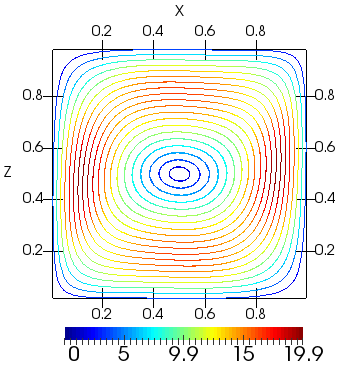
\includegraphics[scale=0.9]{pics/Umag.png}
    \caption{Линии тока для задачи естественной конвекции}
    \label{fig:Nconv}
\end{figure}

\begin{figure}
    \centering
    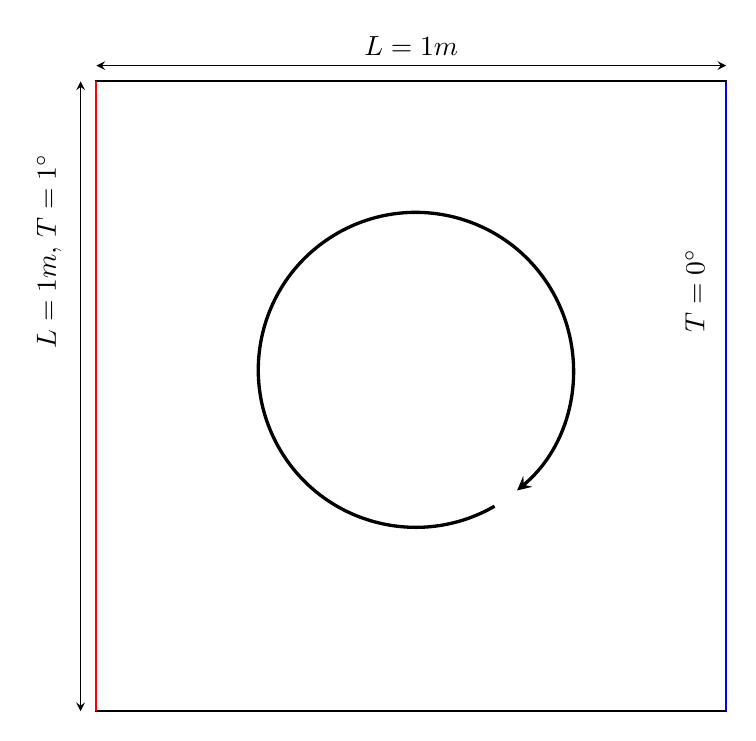
\begin{tikzpicture}[scale = 8]
        \draw[thick] (0,0,0) -- (1,0,0) -- (1,1,0) -- (0,1,0) -- cycle;
        
        \draw[thick, color = red] (0,0,0) -- (0,1,0);
        
        \draw[thick, color = blue] (1,0,0) -- (1,1,0);
        \draw (0.95,0.75) node[left,rotate=90] {$T=0^{\circ}$};
        
        \draw [<->,>=stealth](-0.025,0)--(-0.025,1);
        \draw (-0.075,0.9) node[left,rotate=90] {$L=1 m,$  $T=1^{\circ}$};
        
        \draw [<->,>=stealth](0,1.025)--(1,1.025);
        \draw (0.5,1.025) node[above] {$L=1 m$};
        \draw[ very thick,->, >=stealth] (0.15,0.9)  ++ (-50:.75) arc (300:-50:.25 and .25);
        
    \end{tikzpicture}
    \caption{Схематичное изображение задачи для естественной конвекции}
    \label{fig:convectionScratch}
\end{figure}

\subsection{Валидация}

Аттрактор внутренних волн -- это сложное явление, которое происходит после многократного отражения внутренних волн от стенок резервуара. PISO алгоритмы из предыдущего раздела не справляются с моделированием этого феномена, но результаты моделирования аттрактора с помощью решателя QHDFoam показывают неплохие результаты. Удалось добиться ошибки меньше 3\% см. Рис. \ref{fig:AdamsBashforthEulerNek3D}.

\begin{figure}[hbt!]
    \centering
        
    \begin{tikzpicture}[scale = 1,spy using outlines={circle, magnification=6, connect spies}]
        \begin{axis}
            [scale only axis, xlabel=Линия пробы $m \cdot 10^{-3}$, ylabel=$U_x\;\; m/s \cdot 10^{-3}$, grid=major,legend style={at={(0,1),font=\LARGE},anchor=north west}, ymin=-0.8, ymax=0.8,xmin=0,xmax=20,legend style={nodes={scale=0.5, transform shape}}, x post scale=1.6]

            \addplot[solid,color=black,thick] table [x=Points:1, y=U, col sep=comma] {CSV/NEK5000.csv};
            \addplot[solid,color=red,thick] table [x=Points:1, y=U, col sep=comma] {CSV/QHD480x320.csv};
            \addplot[solid,color=green!60!black,thick] table [x=Points:1, y=U, col sep=comma] {CSV/QHD240x160.csv};
            \addplot[solid,color=blue,thick] table [x=Points:1, y=U, col sep=comma] {CSV/QHD240x1602tau.csv};
            \legend{NEK500,QHDFoam 480x320, QHDFoam 240x160, QHDFoam 240x160 $\tau \cdot 2$}

            \coordinate (spypoint) at (axis cs:14.7,0.7);
            \coordinate (magnifyglass) at (axis cs:15.5,-0.3);
        \end{axis}
        \spy [blue, size=4cm] on (spypoint) in node[fill=white] at (magnifyglass);
    \end{tikzpicture} 
    \caption{Количественное сравнение результатов моделирования}
    \label{fig:AdamsBashforthEulerNek3D}
\end{figure}


Также количественные исследования демонстрируют сходимость решения получаемое с помощью квазигидродинамических уравнений к решению полученному с помощью метода высокого порядка (см. Рис. \ref{fig:tauAttr}) в отличие от результатов полученных с помощью PISO (см. Рис. \ref{fig:PISOattr}).

\begin{figure}
    \centering
        \begin{tikzpicture}[scale = 1.1]
          \begin{axis}
             [scale only axis, grid=major,legend style={at={(0,1),font=\LARGE},anchor=north west}, ymin=-0.8*10^-3, ymax=1.7*10^-3, xmin=0.0,legend style={nodes={scale=0.5, transform shape}}, x post scale=1.5,xlabel={$y$}, ylabel={$U_x$}];
            \addplot[solid,color=red,thick] table [x=Points:1, y=U:0, col sep=comma] {CSV/Ux300.5tau.csv};
            \addplot[solid,color=green,thick] table [x=Points:1, y=-U:0, col sep=comma] {CSV/Ux301tau.csv};
            \addplot[solid,color=blue,thick] table [x=Points:1, y=U:0, col sep=comma] {CSV/Ux302tau.csv};
            %\addplot[solid,color=violet,dashed,thick] table [x=Points:1, y=-U:0, col sep=comma] {CSV/Ux30tau001200sBackward.csv};
            \legend{$\tau = 0.005$,$\tau = 0.01$,$\tau = 0.02$,Adams-Bashforth}
          \end{axis}
          \begin{axis}
            [scale only axis, ymin=-0.8*10^-1, ymax=1.7*10^-1, xmin=0.0,  yticklabels={,,},xticklabels={,,},legend style={at={(0,0.75),font=\LARGE},anchor=north west},legend style={nodes={scale=0.5, transform shape}},x post scale=1.5];
            \addplot[solid,thick] table [x=Points:1, y=x_velocity, col sep=comma] {CSV/Ux30Nek500T200.csv};
            \legend{NEK5000}
          \end{axis}
        \end{tikzpicture} 
    \caption{Распределение скорости вдоль линии AB. Демонстрируется сходимость по $\tau$.}
    \label{fig:tauAttr}
\end{figure}

Помимо точности реализаций алгоритмов на базе пакета OpenFOAM сравнивалась и скорость их работы на 12 ядрах процессоров Intel X5670 (Таб. \ref{tab:perfom}). Наиболее быстрый метод– метод спектральных элементов. Для того чтобы достичь отметки в 100 с модельного времени потребовалось время исполнение чуть больше тысячи секунд. Сравнение с методом спектральных элементов является условным из-за значительных отличий в реализации. Один спектральный элемент состоит из 81 точки интерполяции, поэтому количество спектральных элементов настолько мало. PISO алгоритм отстал от алгоритма на базе квазигидродинамического подхода более чем в полтора раза при одинаковых условиях расчёта. Такое отставание и объясняется наличием коррекционных циклов, которые отсутствуют в квазигидродинамическом подходе. 

\begin{table}[]
    \caption{\label{tab:perfom}Сравнение производительности на процессоре Intel(R) Xeon(R) CPU X5670 2.93 GHz, 100 с модельного времени, с шагом в $5 \cdot 10^{-3}$, опции компиляции -- gcc -O3.}
    
    \begin{tabular}{c|c|c|c|c|c}
        Подход & Время  & Количество  & PIMPLE      & Коррекции  \\
                 & исполнения (с)   &   элементов  & коррекции & неортогональности     \\
        \hline
         &  & 1296 &  &  \\
        Nek5000 & 1037 & Спектральных & 0 & 0 \\
         &  & элементов &  &  \\
        \hline
         &  & 67 500 &  & \\
        PISO & 7630 & Конечных & 3 & 1\\
         &  & элементов &  & \\
        \hline
         &  & 67 500 &  & \\
        QHD & 4479 &  Конечных & 0 & 0\\
         &  & элементов &  & \\
        \hline
    \end{tabular}
    
    \end{table}

\section*{Заключение к главе 2}

В этой главе рассмаотрены способы моделирования аттракторов внутренних волн. Первая часть посвящена обзору существующих коллективов, которые исследуют фокусировку внутренних волн в лабораторных условиях. В главе также описаны экспериментальные установки, которые используются этими коллективами. 

Также освещены методы численного моделирования аттракторов внутренних волн. Метод спектральных элементов очень мощный инструмент высокого порядка. Однако, метод спектральных элементов очень чувствителен к вычислительной сетке и геометрии. Этот метод не подходит для моделирования аттракторов внутренних волн в естественных условиях сложной топологии океанического дна или при наличии примесей описываемых частицами в воде.

Альтернативный метод -- метод конечных объемов. Позволяет проводить численные эксперименты в условиях приближенных к реальным, включая сложную геометрию океанического дна и осаждение примесей. Однако, его реализация на одной из самых популярных платформ не демонстрирует сеточной сходимости и количественного соответствия методу спектральных элементов. Поддерживаемом метод конечных объемов не позволяет достичь той точности, что гарантирует метод спектральных элементов. Стандартные средства популярных инструментов моделирования несжимаемых течений не могут количественно воспроизвести эффекты множественной фокусировки внутренних волн. 

Подход на основе квазигидродинамических уравнений имеет простой вычислительный алгоритм, количественное совпадение результатов с результатами полученными при помощи метода спектральных элементов.

В этой главе рассмотрены аспекты реализации квазигидродинамического подхода, верификации разработанного алгоритма и валидации на примере задачи формирования аттрактора внутренних волн сравниваются результаты работы алгоритма PISO и QHD. Результаты количественно сравнивались с эталонным решением, полученным при помощи метода спектральных элементов.

Анализ полученных результатов позволяет сделать следующие выводы:
\begin{itemize}
    \item На верификационной задаче о моделировании стационарного течения в скошенной каверне оба метода ведут себя одинаково адекватно, наблюдается сеточная сходимость численных результатов, что говорит об устойчивости методов на деформированных сетках.
    \item На задаче о моделировании формирования аттрактора гравитационных внутренних волн QHD алгоритм показывает результаты как количественно, так и качественно воспроизводящие это явление, как на малых, так и на больших временах. Алгоритм PISO воспроизводит явление лишь качественно и только на небольших временах.
    \item QHD алгоритм показывает сеточную сходимость и сходимость по регуляризационному настроечному параметру. PISO алгоритм не демонстрирует сеточной сходимости при сгущении пространственной сетки.
    \item QHD алгоритм, построенный на базе квазигидродинамических уравнений, не требует дополнительных коррекций вычисленных скоростей и давлений в отличие от алгоритма PISO.
    \item OpenFOAM реализация квазигидродинамического подхода показала более высокую производительность на многопроцессорной системе чем реализация алгоритма PISO.
\end{itemize}

Исходя из вышесказанного можно констатировать преимущества алгоритма QHD при моделировании аттракторов внутренних волн по сравнению со стандартными средствами, ранее реализованными в OpenFOAM на базе алгоритма PISO. 

